\documentclass[border=10pt]{standalone}

\usepackage{tikz}
\usepackage{tikzsymbols}
\usetikzlibrary{calc,patterns,shapes.geometric}

\def\centerarc[#1](#2)(#3:#4:#5){\draw[#1] ($(#2)+({#5*cos(#3)},{#5*sin(#3)})$) arc (#3:#4:#5);}

\begin{document}
	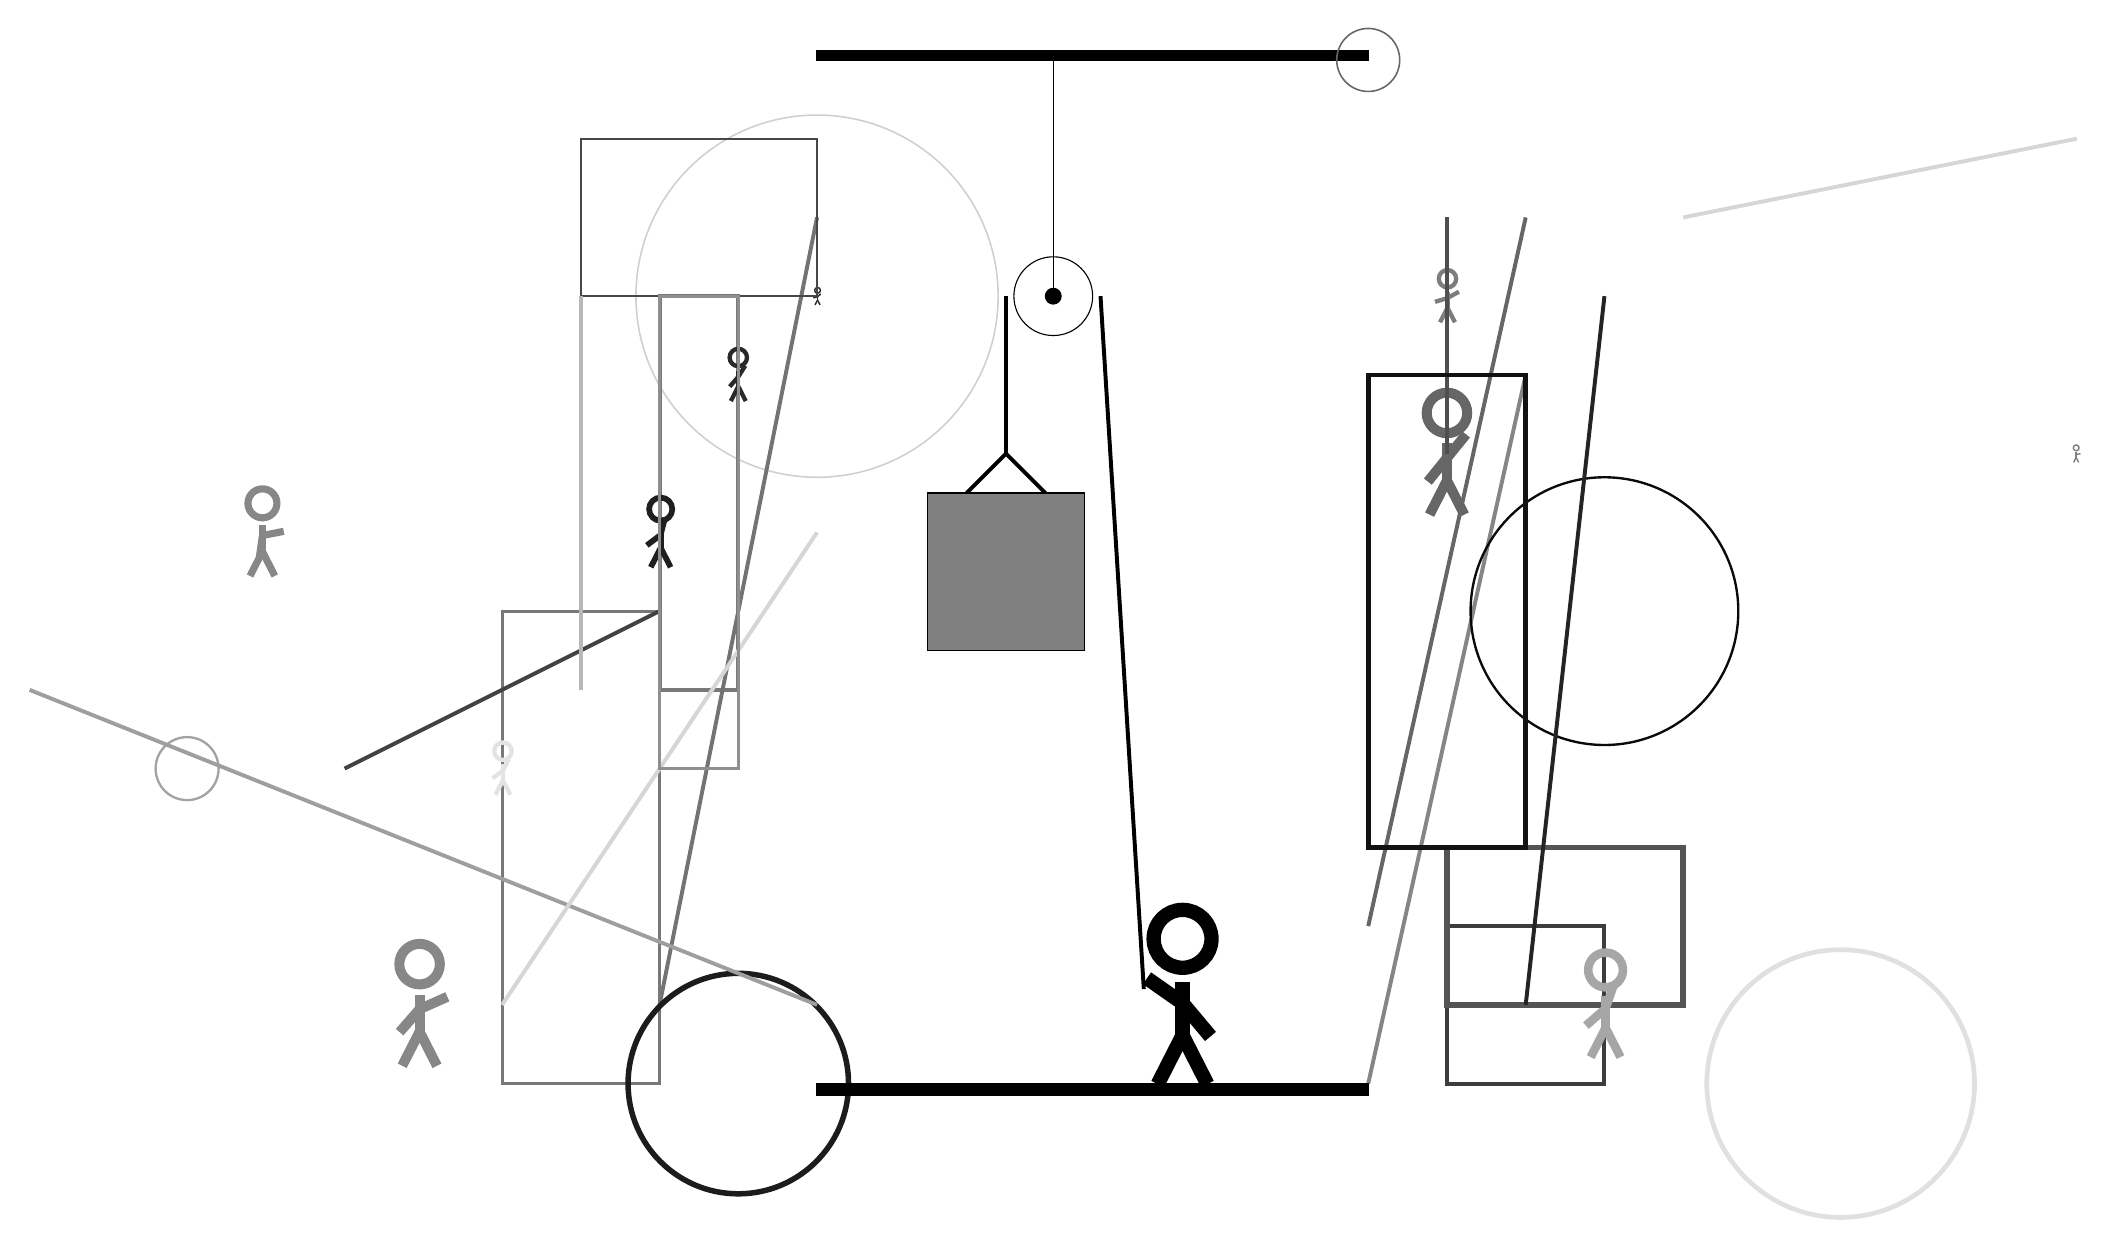
\begin{tikzpicture}
		%%%%% START %%%%%
		
		\draw[fill=black] (-2, 10) rectangle (5, 10.125);
		
		\draw (1, 7) circle (0.5);
		\draw[fill=black] (1, 7) circle (0.1);
		\draw (1, 10) -- (1, 7);
		
		\draw[line width=0.5mm] (-0.1, 4.5) -- (0.4, 5.0) -- (0.9, 4.5);
		\draw[fill=black!50] (-0.6, 4.5) rectangle (1.4, 2.5);
		
		\draw[line width=0.5mm] (0.4, 7) -- (0.4, 5.0);
		\centerarc[line width=0.5mm](1, 7)(0:180:0.6);
		\draw[line width=0.5mm](1.6, 7) -- (2.15, -1.8);
		
		\draw[line width=0.5mm, color=black!60](7, 8) -- (5, -1);
		
		\node[line width=0.5mm, color=black!51] at (6, 7) {\Strichmaxerl[3][17][29]};
		\draw[line width=0.5mm, color=black!76] (6, -1) rectangle (8, -3);
		\node[line width=0.4mm, color=black!60] at (6, 5) {\Strichmaxerl[7][51][51]};
		\draw [line width=0.2mm, color=black!19](-2, 7) circle (2.3);
		\draw[line width=0.5mm, color=black!48](5, -3) -- (7, 6);
		\draw[line width=0.7mm, color=black!67] (6, 0) rectangle (9, -2);
		
		\draw[line width=0.5mm, color=black!53] (-3, 7) rectangle (-4, 2);
		\node[line width=0.4mm, color=black!84] at (-2, 7) {\Strichmaxerl[1][14][43]};
		\draw [line width=0.3mm, color=black!96](8, 3) circle (1.7);
		\draw[line width=0.5mm, color=black!55](-2, 8) -- (-4, -2);
		\node[line width=0.3mm, color=black!47] at (-9, 4) {\Strichmaxerl[5][82][11]};
		\draw [line width=0.2mm, color=black!60](5, 10) circle (0.4);
		
		\node[line width=0.5mm, color=black!88] at (-4, 4) {\Strichmaxerl[4][37][76]};
		\draw[line width=0.5mm, color=black!69](6, 8) -- (6, 5);
		\draw[line width=0.4mm, color=black!53] (-4, -3) rectangle (-6, 3);
		
		\draw[line width=0.5mm, color=black!74](-4, 3) -- (-8, 1);
		
		\draw [line width=0.7mm, color=black!89](-3, -3) circle (1.4);
		\node[line width=0.4mm, color=black!50] at (14, 5) {\Strichmaxerl[1][88][6]};
		
		\draw [line width=0.3mm, color=black!36](-10, 1) circle (0.4);
		\draw[line width=0.5mm, color=black!38](-2, -2) -- (-12, 2);
		
		\draw[line width=0.5mm, color=black!16](-2, 4) -- (-6, -2);
		\node[line width=0.4mm, color=black!47] at (-7, -2) {\Strichmaxerl[7][49][24]};
		\node[line width=0.7mm, color=black!84] at (-3, 6) {\Strichmaxerl[3][49][58]};
		\draw[line width=0.3mm, color=black!72] (-2, 7) rectangle (-5, 9);
		\draw[line width=0.6mm, color=black!93] (5, 0) rectangle (7, 6);
		
		\draw[line width=0.5mm, color=black!28](-5, 2) -- (-5, 7);
		\draw[line width=0.4mm, color=black!44] (-3, 1) rectangle (-4, 7);
		
		\node[line width=0.3mm, color=black!11] at (-6, 1) {\Strichmaxerl[3][37][62]};
		
		\draw [line width=0.6mm, color=black!12](11, -3) circle (1.7);
		\node[line width=0.4mm, color=black!35] at (8, -2) {\Strichmaxerl[6][41][71]};
		
		\draw[line width=0.5mm, color=black!16](9, 8) -- (14, 9);
		\draw[line width=0.5mm, color=black!86](8, 7) -- (7, -2);
		
		
		\node at (2.6, -1.9) {\Strichmaxerl[10][-35][-50]};
		
		\draw[fill=black] (-2, -3) rectangle (5, -3.15);
		
		%%%%% END %%%%%
	\end{tikzpicture}
\end{document}